\documentclass[../practica_04.tex]{subfiles}

\begin{document}

    \begin{enumerate}
        \item 
            \begin{itemize}
                \item $z = f(x,y) = 3y^2-2x^2+x$
                \item $P = (2,-1,-3)$
            \end{itemize}

            \begin{itemize}
                \item $f_x(x,y) = -4x + 1$

                    Que al ser un polinomio es continua en todo R
                \item $f_y(x,y) = 6y$

                    Que al ser un polinomio es continua en todo R
            \end{itemize}

            $ \Rightarrow z - z_0 = f_x(x_0,y_0)(x - x_0) + f_y(x_0,y_0)(y-y_0) =$

            $ z = -7(x - 2) - 6(y+1) - 3 = $

            $ z = -7x -6y + 14 - 6 - 3 $

            $ \Pi: z = -7x -6y + 5 $

            $ 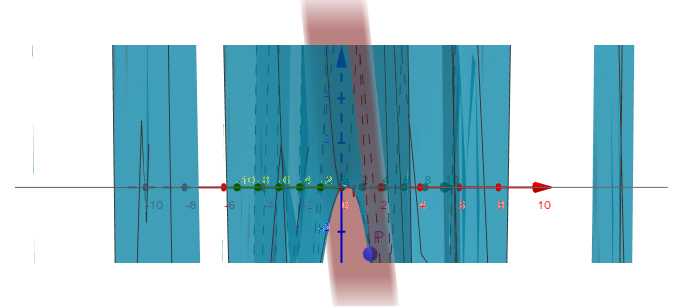
\includegraphics[scale=0.4]{ej09/resources/9a.png}  $

        \item 
            \begin{itemize}
                \item $z = \sqrt{xy}$
                \item $P= (1,1,1)$
            \end{itemize}

            \begin{itemize}
                \item $f_x(x,y) = ((xy)^{\frac{1}{2}})^{\prime} = \frac{1}{2}\cdot (xy)^{-\frac{1}{2}} = \frac{1}{2\sqrt{xy}}$

                    Es continua en (1,1,1) ya que no se anula el denominador

                \item $f_x(x,y) = ((xy)^{\frac{1}{2}})^{\prime} = \frac{1}{2}\cdot (xy)^{-\frac{1}{2}} = \frac{1}{2\sqrt{xy}}$

                    Es continua en (1,1,1) ya que no se anula el denominador
            \end{itemize}

            $ \Rightarrow z - z_0 = f_x(x_0,y_0)(x - x_0) + f_y(x_0,y_0)(y-y_0) =$

            $ z = \frac{1}{2}(x-1) + \frac{1}{2}(y-1) + 1 $

            $ z = \frac{x}{2} + \frac{y}{2} $

            $ 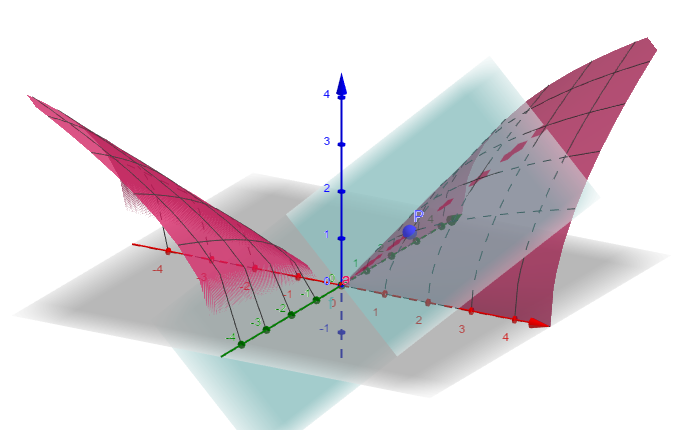
\includegraphics[scale=0.4]{ej09/resources/9b.png}  $

        \item 
            \begin{itemize}
                \item $z = xe^{xy}$
                \item $P = (2,0,2)$
            \end{itemize}

            \begin{itemize}
                \item $f_x(x,y) = e^{xy} + xye^{xy}$
            
                    Es continua en todo ${\real}^2$
                \item $f_y(x,y) = x^2e^{xy}$

                    Es continua en todo ${\real}^2$
            \end{itemize}

            $ \Rightarrow z - z_0 = f_x(x_0,y_0)(x - x_0) + f_y(x_0,y_0)(y-y_0) =$

            $ z = x - 2 + 4y - 2 $

            $ z = x + 4y $

            $ 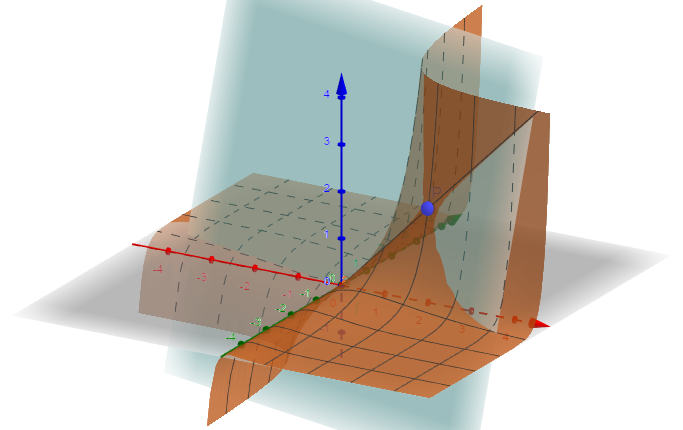
\includegraphics[scale=0.4]{ej09/resources/9c.png}  $

    \end{enumerate}

\end{document}
